\chapter{Perancangan}
\label{chap:perancangan}

Pada bab ini akan dibahas mengenai perancangan perangkat lunak. Perancangan perangkat lunak akan mencakup diagram kelas rinci, perancangan berorientasi objek, dan perancangan antarmuka.

\section{Diagram Kelas Rinci}

Diagram kelas rinci digunakan sebagai gambaran umum untuk setiap kelas yang ada dalam perangkat lunak yang dibangun serta keterkaitan setiap kelas. Diagram kelas rinci dapat dilihat pada Gambar \ref{fig:final_class_diagram}. Ada perbedaan antara diagram kelas pada Gambar \ref{fig:final_class_diagram} dengan kelas diagram pada Bab \ref{chap:analisis}. Pada diagram kelas rinci ditambahkan beberapa atribut dan fungsi sesuai dengan kebutuhan dari masing-masing kelas.

%\clearpage
%diagram
%\begin{sidewaysfigure}[H]
	%\centerline{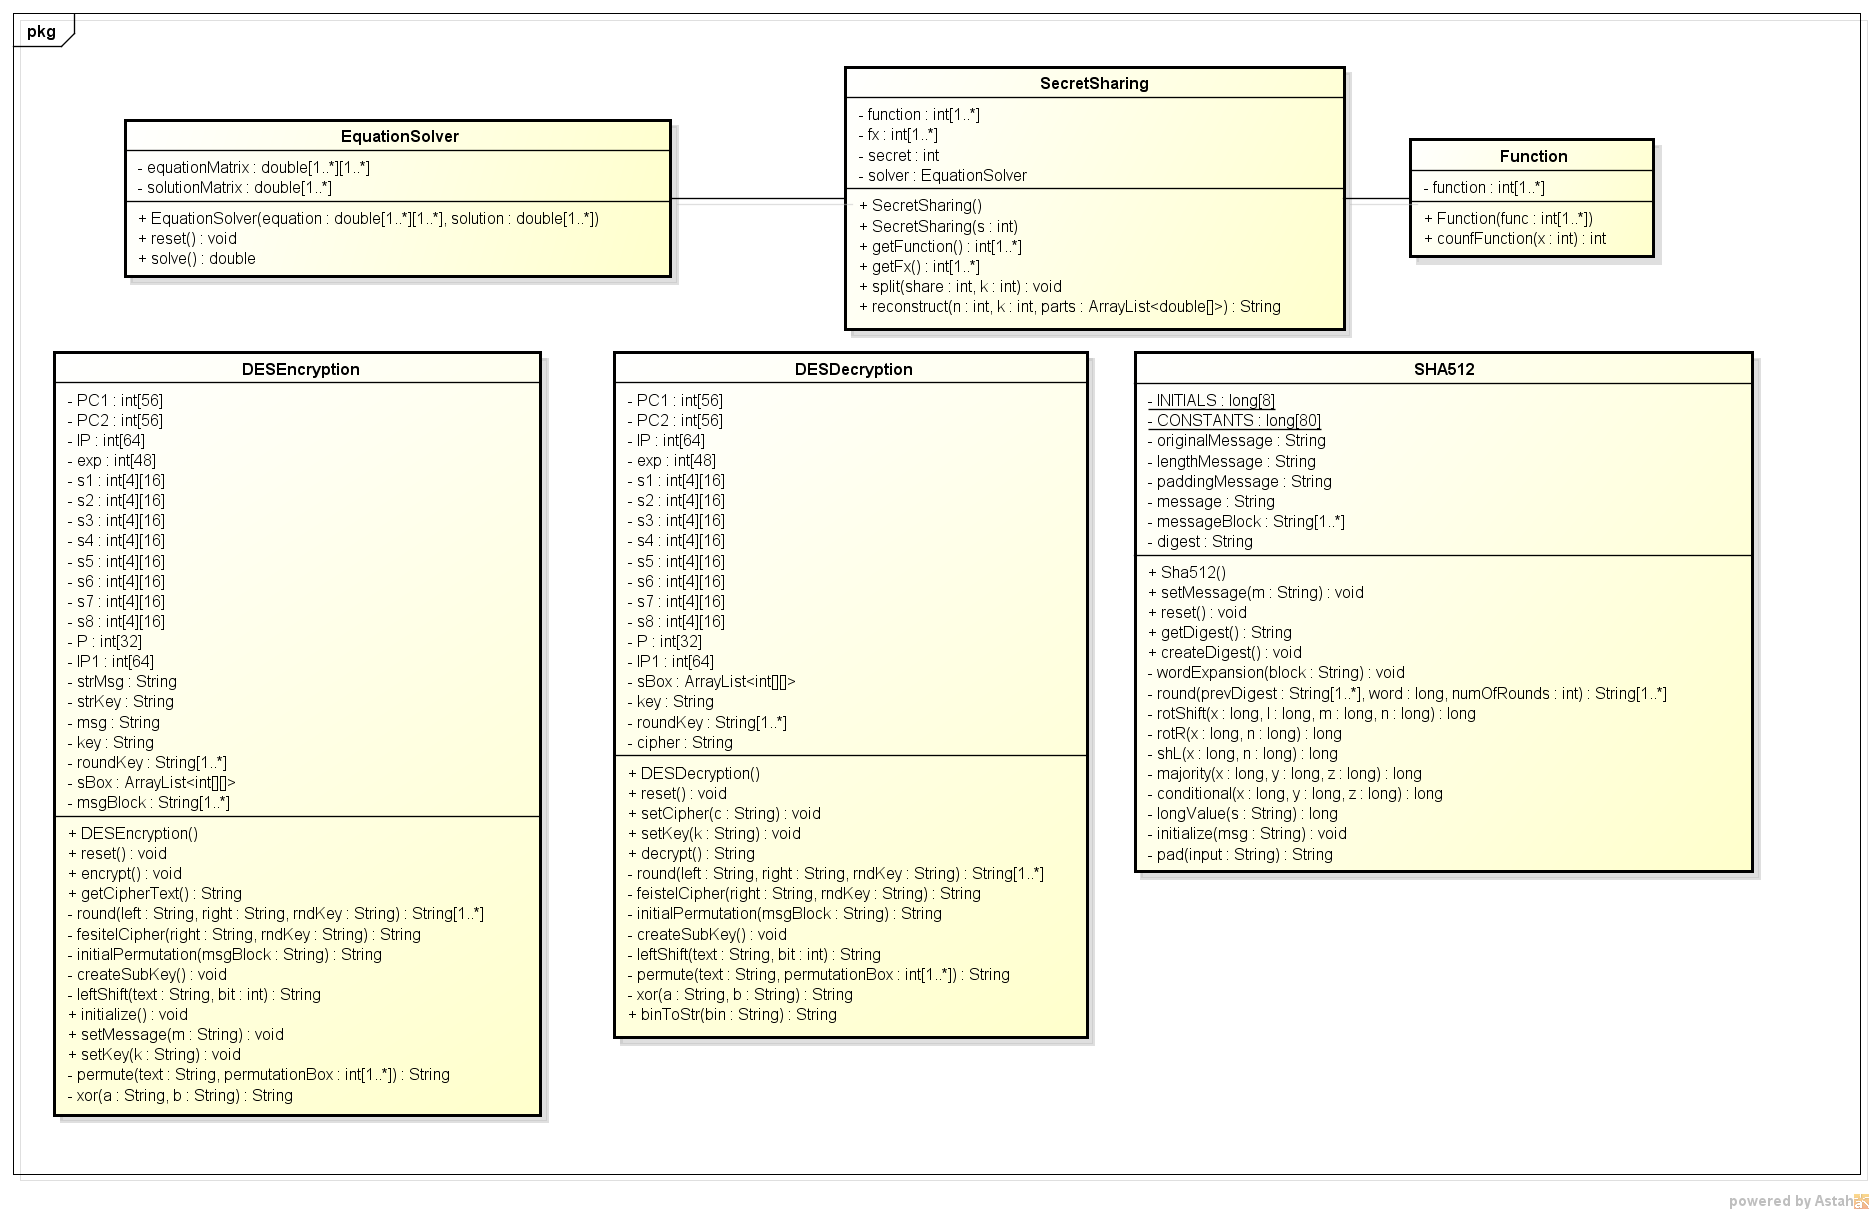
\includegraphics[scale=0.5]{Gambar/final_class_diagram}}
	%\caption{Diagram Kelas Rinci}\label{fig:final_class_diagram}
%\end{sidewaysfigure}

\begin{figure}[h]
	\centering
	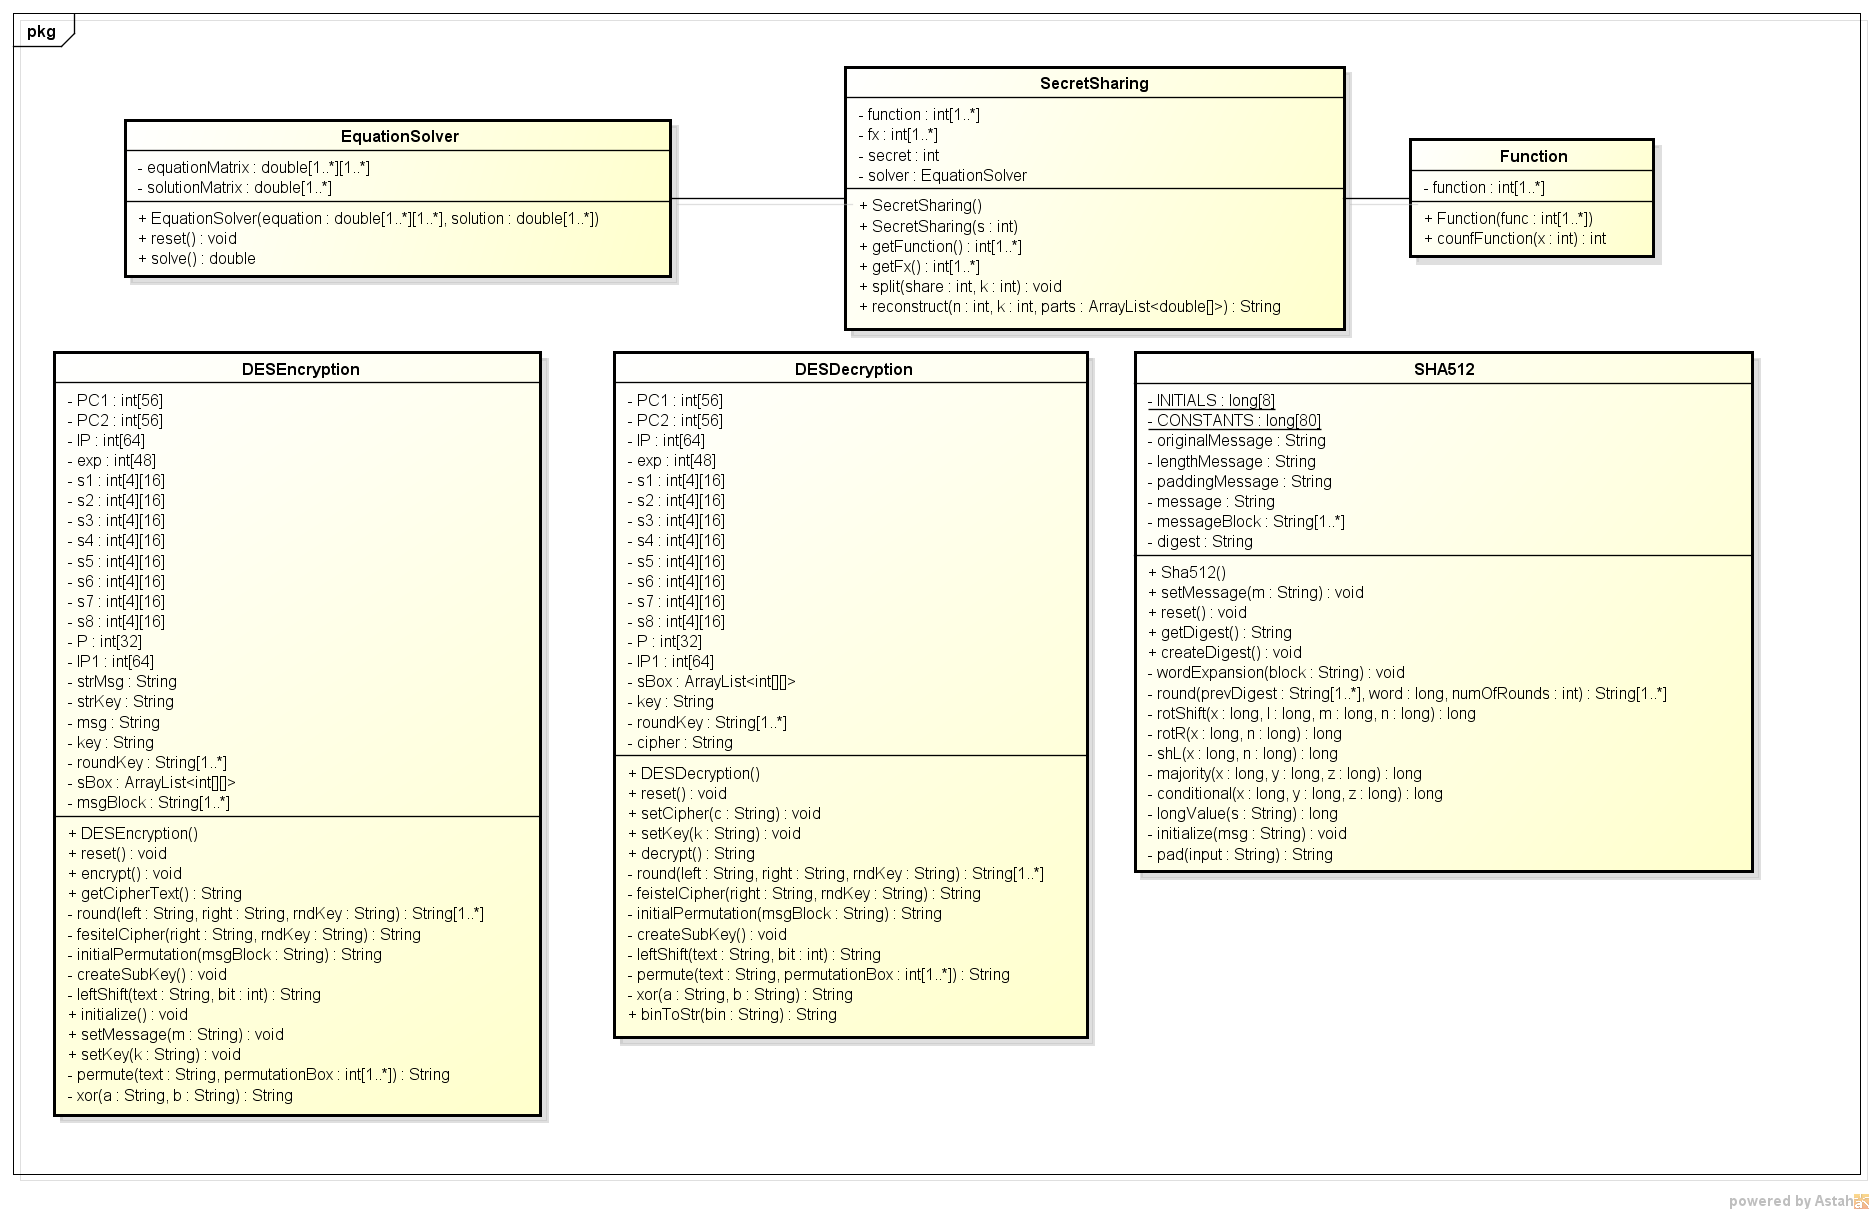
\includegraphics[angle=90, origin=c, scale=0.5]{Gambar/final_class_diagram}
	\caption{Diagram Kelas Rinci}\label{fig:final_class_diagram}
\end{figure}

\section{Deskripsi Kelas dan Fungsi}

Pada bagian ini akan berisi mengenai penjelasan secara rinci masing-masing kelas. Tujuannya adalah menjelaskan peran setiap kelas dalam perangkat lunak yang dibangun.

\subsection{Kelas \textit{SHA512}}

Kelas \textit{SHA512} merupakan kelas yang mengimplementasikan \textit{Secure Hashing Algorithm 512} (SHA-512). Cara kerja algoritma dapat dilihat pada bagian \ref{sec:SHA512}. Kelas SHA512 ditunjukkan pada Gambar \ref{fig:classsha512}.

\begin{figure}[H]
	\centering
	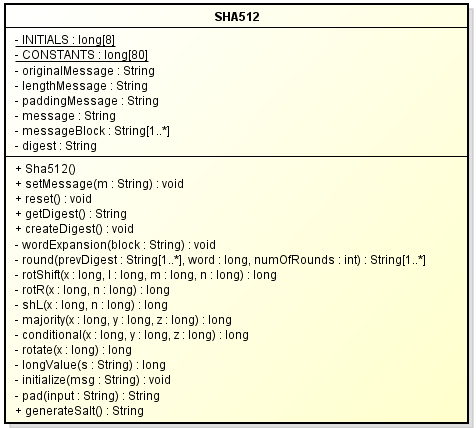
\includegraphics[scale=0.5]{Gambar/class_sha512}
	\caption{Kelas SHA512}\label{fig:classsha512}
\end{figure}

Adapun atribut dari kelas \textit{SHA512}, yaitu \textit{INITIALS, CONSTANTS, originalMessage, lengthMessage, paddingMessage, message, messageBlock,} dan \textit{digest}. Berikut penjelasan masing-masing atribut tersebut:

\begin{enumerate}
	\item \textit{long[8] INITIALS} \\
	Atribut yang berguna untuk menyimpan nilai dari konstanta awal.
	\item \textit{long[80] INITIALS} \\
	Atribut yang berguna untuk menyimpan konstanta yang digunakan dalam setiap putaran SHA-512.
	\item \textit{String originalMessage} \\
	Atribut yang berguna untuk menyimpan \textit{message} yang belum di\textit{padding} dalam bentuk \textit{string} biner.
	\item \textit{String lengthMessage} \\
	Atribut yang berguna untuk menyimpan informasi mengenai panjang atribut \textit{originalMessage} dalam bentuk \textit{string} biner.
	\item \textit{String paddingMessage} \\
	Atribut yang berguna untuk menyimpan blok \textit{padding} dalam bentuk \textit{string} biner.
	\item \textit{String message} \\
	Atribut yang berguna untuk menyimpan \textit{message} yang sudah di\textit{padding} dalam bentuk \textit{string} biner.
	\item String digest \\
	Atribut yang berguna untuk menyimpan \textit{digest} dari atribut \textit{message} dalam bentuk string \textit{biner}.
\end{enumerate}

Adapun fungsi yang membangun kelas \textit{SHA512}, yaitu \textit{Sha512, setMessage, reset, getDigest, wordExpansion, round, rotShift, rotR, shL, majority, conditional, longValue, initialize,} dan \textit{pad}. Berikut penjelasan masing-masing fungsi tersebut:

\begin{enumerate}
	\item \textit{Sha512} \\
	Merupakan konstruktor dari kelas \textit{SHA512}.
	\item \textit{void setMessage(String m)} \\
	Menyimpan nilai \textit{string m} ke dalam atribut \textit{originalMessage}.
	\item \textit{void reset} \\
	Mengembalikan nilai atribut \textit{originalMessage, lengthMessage, paddingMessage, message,} dan \textit{digest} menjadi \textit{string} kosong dan mengembalikan nilai atribut \textit{messageBlock} menjadi \textit{array string} kosong.
	\item \textit{String getDigest} \\
	Mengembalikan \textit{string digest} dalam bentuk heksadesimal.
	\item \textit{void createDigest} \\
	Membuat \textit{digest} dari \textit{message}. Algoritma untuk membuat digest ini dapat dilihat pada bagian \ref{sec:SHA512}.
	\item void wordExpansion(String block)
\end{enumerate}

\subsection{Kelas \textit{Function}}

Kelas \textit{Function} merupakan kelas yang merepresentasikan sebuah fungsi polinomial \begin{math}f(x)\end{math}. Kelas \textit{Function} ditunjukkan pada Gambar \ref{fig:classfunction}.

\begin{figure}[H]
	\centering
	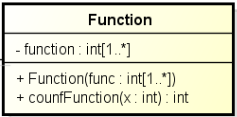
\includegraphics[scale=0.7]{Gambar/class_function}
	\caption{Kelas \textit{Function}}\label{fig:classfunction}
\end{figure}

Adapun atribut dari kelas \textit{Function} adalah \textit{function}. Atribut \textit{function} berguna untuk menyimpan nilai setiap koefesien dari fungsi polinomial \begin{math}f(x)\end{math} dalam tipe data \textit{array} bilangan bulat.

Sementara itu, fungsi yang dimiliki oleh kelas \textit{Function}, yaitu \textit{Function} dan \textit{countFunction}. Berikut penjelasan masing-masing fungsi:

\begin{enumerate}
	\item \textit{Function(int[] func)} \\
	Merupakan konstruktor dari kelas \textit{Function} yang menerima masukan \textit{array} bilangan bulat.
	\item \textit{int countFunction(int x)} \\
	Menghitung nilai \begin{math}x\end{math} untuk fungsi polinomial \begin{math}f(x)\end{math}. Algoritma dari fungsi ini ditunjukkan pada Algoritma \ref{countFunction}.
	\begin{algorithm}
		\caption{countFunction}
		\label{countFunction}
		\begin{algorithmic}[1]
			\Function{countFunction}{x}
				\For{i < panjang\: array\: dari\: atribut\: function}
					\State \begin{math}res = res + (function[i]\: \cdot\: x^i)\end{math}
				\EndFor
				\State return \begin{math}res\end{math}
			\EndFunction
		\end{algorithmic}
	\end{algorithm}
\end{enumerate}

\subsection{Kelas \textit{EquationSolver}}

Kelas \textit{EquationSolver} adalah kelas yang mengimplementasikan eliminasi Gauss-Jordan (Bagian \ref{sec:eliminasigaussjordan}). Kelas ini berperan untuk menyelesaikan persamaan linear. Gambar \ref{fig:classequationsolver} menunjukkan kelas \textit{EquationSolver}.

\begin{figure}[H]
	\centering
	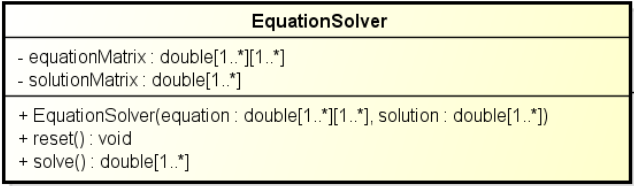
\includegraphics[scale=0.7]{Gambar/class_equation_solver}
	\caption{Kelas \textit{EquationSolver}}\label{fig:classequationsolver}
\end{figure}

Adapun atribut dari kelas \textit{EquationSolver} yaitu, \textit{equationMatrix} dan \textit{solutionMatrix}. Berikut penjelasan masing-masing atribut:

\begin{enumerate}
	\item \textit{double[][] equationMatrix} \\
	Atribut yang menyimpan bentuk matriks dari persamaan linear.
	\item \textit{double[] solutionMatrix} \\
	Atribut yang menyimpan bentuk matriks dari solusi masing-masing persamaan linear.
\end{enumerate}

Sementara itu, fungsi yang dimiliki oleh kelas \textit{EquationSolver} yaitu, \textit{EquationSolver}, \textit{reset}, dan \textit{solve}. Berikut penjelasan masing-masing fungsi:

\begin{enumerate}
	\item \textit{EquationSolver(double[][] equation, double[] solution)} \\
	Merupakan konstruktor dari kelas \textit{EquationSolver} yang menerima masukan berupa matriks persamaan dan matriks solusi.
	\item \textit{void reset} \\
	Mengembalikan nilai atribut \textit{equationMatrix} dan \textit{solutionMatrix} menjadi \textit{array} kosong.
	\item double[] solve \\
	Mencari solusi dari persamaan linear dan mengembalikan solusi dalam bentuk \textit{array}.
\end{enumerate}

\subsection{Kelas \textit{SecretSharing}}

\subsection{Kelas \textit{DESEncryption}}

\subsection{Kelas \textit{DESDecryption}}

\subsection{Kelas \textit{DataReader}}

Kelas \textit{DataReader} merupakan kelas yang berperan untuk membaca berkas teks. Kelas \textit{DataReader} ditunjukkan pada Gambar \ref{fig:classdatareader}.

\begin{figure}[H]
	\centering
	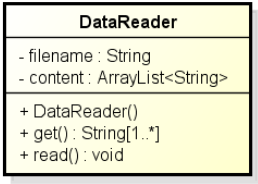
\includegraphics[scale=0.8]{Gambar/class_data_reader}
	\caption{Kelas \textit{DataReader}}\label{fig:classdatareader}
\end{figure}

Kelas ini memiliki 2 atribut, yaitu \textit{filename} dan \textit{content}. Berikut penjelasan masing-masing atribut:

\begin{enumerate}
	\item \textit{String filename} \\
	Atribut yang menyimpan nama dari berkas teks yang dibaca.
	\item \textit{ArrayList<String> content} \\
	Atribut yang menyimpan isi dari berkas teks yang dibaca.
\end{enumerate}

Adapun kelas ini memiliki 3 fungsi, yaitu \textit{DataReader, get,} dan \textit{read}. Berikut penjelasan masing-masing fungsi:

\begin{enumerate}
	\item \textit{DataReader} \\
	Merupakan konstruktor dari kelas \textit{DataReader}.
	\item \textit{String[] get} \\
	Fungsi yang berguna untuk mengembalikan atribut \textit{content}.
	\item \textit{void read} \\
	Fungsi yang berperan membaca berkas teks.
\end{enumerate}

\subsection{Kelas \textit{DataWriter}}

Kelas \textit{DataWriter} adalah kelas yang berperan untuk menulis keluaran ke dalam berkas teks. Kelas \textit{DataWriter} ditunjukkan pada Gambar \ref{fig:classdatawriter}.

\begin{figure}[H]
	\centering
	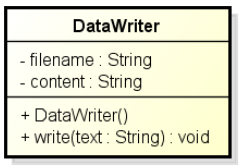
\includegraphics[scale=0.8]{Gambar/class_data_writer}
	\caption{Kelas \textit{DataWriter}}\label{fig:classdatawriter}
\end{figure}

Kelas ini memiliki 2 atribut, yaitu \textit{filename} dan \textit{content}. Berikut penjelasan masing-masing atribut:

\begin{enumerate}
	\item \textit{String filename} \\
	Atribut yang menyimpan nama dari berkas teks yang akan ditulis.
	\item \textit{String content} \\
	Atribut yang menyimpan isi dari berkas teks yang akan ditulis.
\end{enumerate}

Adapun kelas ini memiliki 2 fungsi, yaitu DataWriter dan write. Berikut penjelasan masing-masing fungsi:

\begin{enumerate}
	\item DataWriter \\
	Merupakan konstruktor dari kelas \textit{DataWriter}.
	\item \textit{write(String text)} \\
	Fungsi yang berperan untuk menulis isi dari berkas teks.
\end{enumerate}

\section{Perancangan Antarmuka}

Perangkat lunak yang dikembangkan akan memiliki 3 tampilan utama, tampilan untuk menyimpan \textit{password}, tampilan untuk mengembalikan \textit{password}, dan tampilan untuk memilih menyimpan \textit{password} atau mengembalikan \textit{password}.

Gambar \ref{fig:tampilan-awal} menunjukkan tampilan awal yang akan dimunculkan pertama kali untuk memilih menyimpan \textit{password} atau mengembalikan \textit{password}.

%diagram
\begin{figure}[H]
	\centerline{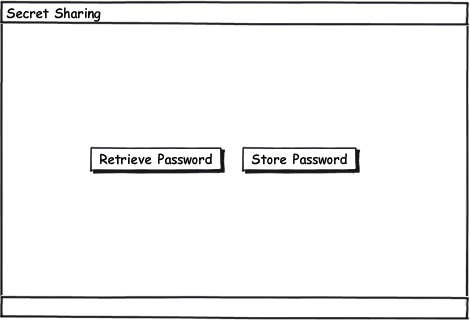
\includegraphics[scale=0.5]{Gambar/tampilan-utama}}
	\caption{Perancangan Tampilan Awal}\label{fig:tampilan-awal}
\end{figure}

Tampilan utama ini cukup sederhana. Dalam tampilan utama pada Gambar \ref{fig:tampilan-awal}, hanya terdapat 2 pilihan, yaitu \textit{store password} untuk menyimpan \textit{password} dan \textit{retrieve password} untuk mengembalikan \textit{password}. Selanjutnya, jika pengguna memilih \textit{store password}, maka akan ditampilkan halaman \textit{store password}.

%diagram
\begin{figure}[H]
	\centerline{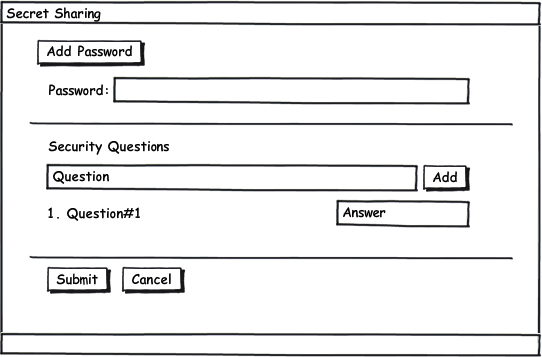
\includegraphics[scale=0.5]{Gambar/store_password}}
	\caption{Perancangan Tampilan Menyimpan \textit{Password}}\label{fig:store_password}
\end{figure}

Pada tampilan menyimpan \textit{password} di Gambar \ref{fig:store_password}, tombol "\textit{Add Password}" berfungsi untuk menambah \textit{text box password}, pada bagian ini pengguna bisa mengisi \textit{password} yang akan disimpan. Bagian "\textit{Security Questions}" berisi pertanyaan keamanan yang dibuat oleh pengguna. Setelah pengguna mengisi pertanyaan personal pada \textit{text box} di bagian "\textit{Security Questions}" dan menekan tombol "\textit{Add}", akan muncul pertanyaan yang sudah dibuat, kemudian pengguna harus mengisi jawaban dari pertanyaan keamanan yang sudah dibuat.

Setelah mengisi seluruh pertanyaan keamanan, pengguna bisa menyimpan \textit{password} dengan menekan tombol "\textit{Submit}". Tombol "\textit{Cancel}" berfungsi untuk kembali ke tampilan awal. Setelah tombol "\textit{Submit}" ditekan, maka \textit{password} sudah disimpan dan akan kembali ditampilkan tampilan awal.

Berikutnya adalah tampilan untuk mengembalikan \textit{password}. Gambar \ref{fig:retrieve_password} menunjukkan tampilan untuk mengembalikan \textit{password}.

%diagram
\begin{figure}[H]
	\centerline{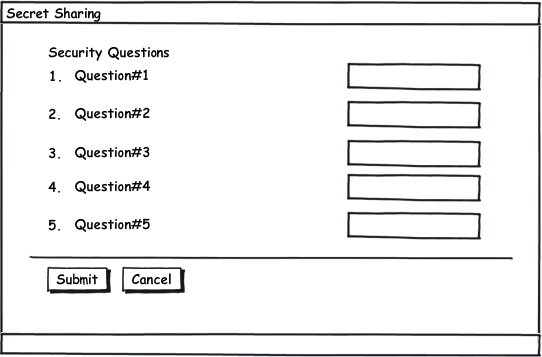
\includegraphics[scale=0.5]{Gambar/retrieve_password}}
	\caption{Perancangan Tampilan Mengembalikan \textit{Password}}\label{fig:retrieve_password}
\end{figure}

Pada bagian untuk mengembalikan \textit{password}, tampilannya cukup sederhana dan pengguna hanya cukup memasukkan setiap jawaban dari pertanyaan keamanan yang sudah dibuat sebelumnya di bagian penyimpanan password. Pada bagian ini, pengguna bebas untuk memilih mengisi setiap pertanyaan atau tidak menjawab pertanyaan keamanan. Setelah seluruh pertanyaan sudah dijawab, pengguna dapat menekan tombol "\textit{Submit}" yang kemudian akan menunjukkan \textit{password} pengguna.

Gambar \ref{fig:password} menunjukkan tampilan sesudah pengguna menekan tombol "\textit{Submit}" pada bagian di Gambar \ref{fig:retrieve_password}.

%diagram
\begin{figure}[H]
	\centerline{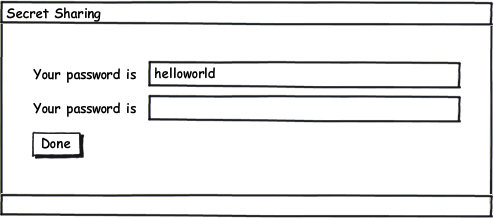
\includegraphics[scale=0.5]{Gambar/password}}
	\caption{Perancangan Tampilan Mengembalikan \textit{Password}}\label{fig:password}
\end{figure}

Jika banyak pertanyaan keamanan yang dijawab benar oleh pengguna sesuai dengan minimal banyak pertanyaan keamanan yang dijawab benar maka pengguna bisa melihat \textit{password} yang sudah disimpan. Tapi, jika banyak pertanyaan keamanan yang dijawab benar oleh pengguna kurang dari minimal banyak pertanyaan keamanan yang harus dijawab benar maka pengguna tidak bisa melihat \textit{password} yang sudah disimpan.